\documentclass[12pt]{article}
\usepackage[margin=1.27cm]{geometry}
\usepackage{setspace}
\usepackage{fontspec}
% \usepackage[T1]{fontenc}
% \usepackage[utf8]{inputenc}
\usepackage{amsmath,txfonts,amssymb,nicefrac,mathtools,pifont} %for math
\usepackage{array,tabularx,multirow,fmtcount} %for tables
\usepackage{tikz, pgfplots} %for diagram
\usepackage{multicol} %for multiple column
\usepackage{enumerate,enumitem,adjustbox} %for ordered list
\usepackage{graphicx,subcaption,wrapfig,tcolorbox} %for figure
\usepackage{xparse} %for commands & environments
\usepackage{lipsum} %miscellaneous
\usepackage{colortbl,xcolor,soul} %for default table & border

% #ANCHOR Font settings
\setmainfont{Oxygen}
\newfontfamily\banglafont[Script=Bengali]{Baloo Da 2}
\newfontfamily{\lstsansserif}{IBM Plex Mono}
\renewcommand{\normalsize}{\fontsize{11.5pt}{13pt}\selectfont}


\setlength{\arrayrulewidth}{0.35 pt}
\definecolor{border}{HTML}{A1A1AA}
\arrayrulecolor{border}


% #ANCHOR Document settings
\linespread{1.45}
\setlength\parindent{0pt}
\setlength\parskip{16pt}
\setlist[enumerate]{noitemsep}
\usetikzlibrary{shapes.geometric,decorations.pathreplacing,trees,arrows,positioning,shapes,fit,calc,decorations.markings, decorations.text}
\tikzset{every node/.append style={font=\footnotesize}}
\usepgfplotslibrary{fillbetween}
\pgfdeclarelayer{background}
\pgfsetlayers{background,main}
\pgfplotsset{compat=1.18}
\columnseprule=1pt
\everymath{\displaystyle}
% #ANCHOR Hypernation
\tolerance=1
\emergencystretch=\maxdimen
\hyphenpenalty=10000
\hbadness=10000
\newlength{\colWidth}



% #ANCHOR Colors
\definecolor{azure(colorwheel)}{rgb}{0.0, 0.5, 1.0}
\definecolor{carminepink}{rgb}{0.92, 0.3, 0.26}
\definecolor{orange}{rgb}{0.9, 0.55, 0.22}
\definecolor{violet}{rgb}{0.60, 0.45, 1}
% Syantax Highlighting Colors
\definecolor{keyword}{HTML}{D73A4A}
\definecolor{number}{HTML}{015CC5}
\definecolor{comment}{HTML}{6A737D}
\definecolor{string}{HTML}{1D825E}
\definecolor{function}{HTML}{743FD1}
\definecolor{orange}{HTML}{CF7842}
\definecolor{codeblack}{HTML}{24292F}
\definecolor{divider}{HTML}{A1A1AA}
\definecolor{border}{HTML}{D1D1D1}


% #ANCHOR Ordered & Unordered List
\setlist[itemize,1]{left=0cm, label={\textbullet}}
\setlist[itemize,2,3,4,5,6,7,8,9,10]{left=0.6cm, label={\textbullet}}
\setlist[enumerate,1]{left=0cm}
\setlist[enumerate,2,3,4,5,6,7,8,9,10]{left=0.6cm}
\setul{0.5ex}{0.125ex}



% #ANCHOR Colored Box
\let\oldul\ul
\renewcommand{\ul}[2][keyword]{\text{\setulcolor{#1}\oldul{#2}}}
\newcommand{\redbox}[1]{%
{\color{red}\fbox{\color{black}#1}}
}
\newcommand{\red}[1]{%
\textcolor{red}{#1}
}
\newcommand{\redeq}[1]{%
\text{\color{red}$#1$}
}
\newcommand{\mred}[1]{%
\textcolor{keyword}{#1}
}
\newcommand{\mredeq}[1]{%
\textcolor{keyword}{$#1$}
}
\newcommand{\blue}[1]{%
% {\color{number}#1\hspace{-0.4ex}}
\textcolor{number}{#1}
}
\newcommand{\blueeq}[1]{%
\text{\color{number}$#1$}
}
\newcommand{\cyanbox}[1]{%
{\color{teal}\fbox{\textcolor{black}{#1}}}
}
\newcommand{\cyan}[1]{%
\textcolor{teal}{#1}
}
\newcommand{\pink}[1]{%
\textcolor{magenta}{#1}
}
\newcommand{\orange}[1]{%
\textcolor{orange}{#1}
}
\newcommand{\violet}[1]{%
{\color{violet}#1}
}
\newcommand{\cyaneq}[1]{%
\text{\color{teal}$#1$}
}
\newcommand{\gray}[1]{%
\textcolor{comment}{#1}
}
\newcommand{\pinkeq}[1]{%
\text{\color{magenta}$#1$}
}
\renewcommand{\columnseprulecolor}{\color{divider}}




% #ANCHOR Tabular commands
\newcolumntype{P}[1]{>{\centering\arraybackslash}p{#1}}
\newcolumntype{M}[1]{>{\centering\arraybackslash}m{#1}}
\newcolumntype{C}{>{\centering\arraybackslash}X}
\newcommand{\rspan}[2]{\multirow{#1}{*}{#2}}
\newcommand{\thc}[1]{%
\multicolumn{1}{|c|}{\textbf{#1}}
}
\newcommand{\thcx}[1]{%
\multicolumn{1}{|C|}{\textbf{#1}}
}
\newcommand{\thl}[1]{%
\multicolumn{1}{|l|}{\textbf{#1}}
}
\newcommand{\thr}[1]{%
\multicolumn{1}{|r|}{\textbf{#1}}
}
% Adjusting arraystretch to modify vertical padding
\renewcommand{\arraystretch}{1.25}
% Adjusting tabcolsep to modify horizontal padding
\setlength{\tabcolsep}{10pt}



% #ANCHOR Math commands
\newcommand{\set}[1]{\{$#1$\}}
\newcommand{\tabs}{\ \ \ \ \ \ }
\newcommand{\tab}{\ \ \ }
\newcommand{\cmark}{\ding{51}}%
\newcommand{\xmark}{\ding{55}}%
\newcommand{\boldi}[1]{\boldsymbol{#1}}%
\newcommand{\wspace}{\ \ = \ \ }



% #ANCHOR New commands
\newcommand{\Title}[1]{%
   \begin{center}
      \textbf{\Large{#1}}
   \end{center}
}
\newcommand{\Heading}[1]{%
   \par\vspace{\dimexpr -\baselineskip + 16pt}
   {\fontsize{12pt}{13pt}\selectfont\textbf{#1}}
   \par\vspace{\dimexpr -\baselineskip + 6pt}
}
\newcommand{\BuleHeading}[1]{%
   \par\vspace{\dimexpr -\baselineskip + 16pt}
   {\fontsize{12pt}{13pt}\selectfont\textbf{\textcolor{number}{#1}}}
   \par\vspace{\dimexpr -\baselineskip + 6pt}
}
\newcommand{\CHeading}[1]{%
   \par\vspace{\dimexpr -\baselineskip + 16pt}
   \hspace{\fill}
   {\fontsize{12pt}{13pt}\selectfont\textbf{#1}}
   \hspace{\fill}
   \par\vspace{\dimexpr -\baselineskip + 6pt}
}
\newcommand{\Section}[1]{%
   \par\vspace{\dimexpr -\baselineskip + 16pt}
   \hspace{\fill}
   {\fontsize{13pt}{13pt}\selectfont\textbf{#1}}
   \hspace{\fill}
   \par\vspace{\dimexpr -\baselineskip + 6pt}
}
\newcommand{\seteqno}[1]{%
   \ \cdots \ \cdots \ \cdots \ (#1)
}
\newcommand{\eqor}{%
   \Rightarrow \ \ 
}
\newcommand{\tsub}[1]{%
\textsubscript{#1}\hspace{-0.45ex}
}
\newcommand{\tsup}[1]{%
\textsuperscript{#1}\hspace{-0.45ex}
}
\newcommand{\cbox}[2][cyan]{
\tikz\node[draw=#1,circle,inner sep=2pt,baseline=(a.base)](a){#2};
}
\newcommand{\hrline}{%
\vspace{1ex} {\color{gray}\hrule} \vspace{4ex}
}
\newcommand{\divideX}[1][divider]{{\hspace{1ex}\color{#1}{\vrule}\hspace{1ex}}}
\newcommand{\Reference}[2][Reference]{

\vspace{-0.5\baselineskip}
\begin{center}
   {\fontspec{Merriweather}\textbf{#1:} \textit{#2}} 
\end{center}
}
\newcommand{\bn}[1]{%
   {\banglafont #1}
}

\NewDocumentCommand{\Column}{O{0.49} O{1.5em} m m}{
   \setlength{\colWidth}{\linewidth-#1\linewidth-#2}
   \begin{minipage}[t]{#1\linewidth}
      \noindent
         #3
      \end{minipage}\hspace{\fill}{\color{divider}\vrule width 0.35pt}\hspace{\fill}
      \begin{minipage}[t]{\colWidth}
      \noindent
         #4
   \end{minipage}
}



\begin{document}
\Lecture{Chemistry Final Exam Note}

\Heading{\cyan{Periodic Table}} %/*ANCHOR Periodic

\vspace{-0.5\baselineskip}
\Topic{2. How can you determine the position of an element in the periodic table.}
\ \ Period: The valence shell / last shell of an atom determines the period.

\begin{tabular}{lll}
 Group:&s&: s \bn{এর} power \bn{যত তত}\\
 &p&: $\text{p}+12$\\
 &d&: $\text{d}+\text{s}$\\
 &f&: 3
\end{tabular}

\begin{tabular}{llll}
   \textbf{Atom} & 
   \textbf{Electron configuration} & \textbf{Period} & \textbf{Group}\\
   \text{Na (11)} &$\rightarrow \  \text{1s}^\text{2} \text{2s}^{2} \text{2p}^\text{6} \text{3s}^{\text{\mred{1}}}$ & $3$ & $1$\\
   \text{Cl (17)} &$\rightarrow \  \text{1s}^\text{2} \text{2s}^{2} \text{2p}^\text{6} \text{3s}^\text{2} \text{3p}^{\text{\mred{5}}}$ & $3$ & $5+12=17$ \\
   \text{Ar (18)} &$\rightarrow \  \text{1s}^\text{2} \text{2s}^{2} \text{2p}^\text{6} \text{3s}^\text{2} \text{3p}^{\text{\mred{6}}}$ & $3$ & $6+12=18$ \\
   \text{Cr (24)} &$\rightarrow \  \text{1s}^\text{2} \text{2s}^{2} \text{2p}^\text{6} \text{3s}^\text{2} \text{3p}^\text{6} \text{3d}^{\text{\mred{5}}} \text{4s}^{\text{\mred{1}}}$ & $4$ & $5+1=6$ \\
   \text{Ni (28)} &$\rightarrow \  \text{1s}^\text{2} \text{2s}^{2} \text{2p}^\text{6} \text{3s}^\text{2} \text{3p}^\text{6} \text{3d}^{\text{\mred{8}}} \text{4s}^{\text{\mred{2}}}$ & $4$ & $8+2=10$  \\
   \text{Cu (29)} &$\rightarrow \  \text{1s}^\text{2} \text{2s}^{2} \text{2p}^\text{6} \text{3s}^\text{2} \text{3p}^\text{6} \text{3d}^{\text{\mred{10}}} \text{4s}^{\text{\mred{1}}}$ & $4$ & $10+1=11$  \\
   \text{Ce (58)} &$\rightarrow \ [\text{Xe (54)}] \ \text{4s}^\text{2} \text{6f}^\text{2}$ & $6$ & $3$
\end{tabular}

\vspace{3ex}
\Topic{3. Write a short note on the following:}
\Topic{Metals}
Metals are elements that are typically shiny, malleable, and ductile with high melting and boiling points. They readily lose electrons to form positive ions and have mobile particles that can conduct thermal and electrical energy. Metals are usually found on the left side and at the center of the periodic table and are approximately three-fourths of the discovered elements. Metallic character increases from top to bottom in a group, but decreases from left to right across a period. Group 1A and 2A elements are highly reactive.

\Topic{Metalloids}
Metalloids are elements that exhibit characteristics of both metals and nonmetals. They are solid and have a metallic appearance, but their chemical properties are more like nonmetals. They are brittle and have lower melting and boiling points than metals. Metalloids are typically semiconductors, meaning they conduct electricity better than nonmetals but not as well as metals. They are located along the diagonal line between metals and nonmetals on the periodic table.

\Topic{Non-metals}
Non-metals are a group of elements on the upper right corner of the periodic table that do not possess the typical properties of metals. It means they are not hard, shiny, malleable, ductile, and tend to be brittle, with low melting and boiling points. They tend to form negative ions by accepting or gaining electrons. Non-metals are usually poor conductors of heat and electricity. Among the 22 non-metals, 11 are gases, 1 is a liquid, and 10 are solids.


\Topic{Transition metals}
Transition metals are metallic elements with partially filled d orbitals that can form stable cations with incompletely filled d orbitals. They exhibit metallic properties like luster, malleability, and ductility, with high melting points. They can have various oxidation states and form colored compounds, and are often paramagnetic. They are located in the center of the periodic table.

\Topic{Why are d-block elements colorful?}
% When visible light strikes a transition metal complex or ion, the unpaired electrons in the lower energy (gound state) d-orbitals are promoted to higher energy (exited state) d-orbitals, a process is known as the d-d transition. Since the energy involved in the d-d transition is quantized, only a specific wavelength is absorbed, while the rest of the visible spectrum is transmitted. As a result, transmitted light has a complementary colour to the absorbed colour.
D-block elements have partially filled d-orbitals, which can absorb energy in the form of visible light. When light is absorbed, the unpaired electrons in the lower energy (gound state) d-orbitals are promoted to higher energy (exited state). This transitions are called d-d transitions. The energy difference between the ground and excited states determines which wavelengths of light are absorbed, while the rest of the visible spectrum is transmitted. As a result, transmitted light has a complementary colour to the absorbed colour.

\pagebreak
\Topic{4. Identify the metals, metalloids, transition metals, noble gases and non-metals from the given elements with appropriate explanation. Also mention the group and period of each.}

\vspace{-0.25\baselineskip}
\begin{center}
   \textbf{Na, Al, F, Si, Ge, Ar, Kr, Ag, Au, Zn, K, Sc, Cr, Fr, P, S, Mn}
\end{center}
% Na, Al, F, Ar, Kr, Ag, Au, Zn, K, Sc, Cr, Fr, P, S, Mn
% Si, Ge,




\pagebreak %/*ANCHOR Bonding
\vspace*{-2\baselineskip}
\Heading{\cyan{Chemical bonding}}

\Topic{3. CH\tsub{4}, NH\tsub{3} and H\tsub{2}O have tetrahedral geometry yet their bond angles are different. Why?}
It can be explained by VSEPR theory. According to this theory, even though the hybridization is the same, the repulsive force between the bond pairs and lone pairs is not the same.

\begin{center}
   Bond pair - Bond pair < Bond pair - Lone pair < Lone pair - Lone pair
\end{center}

So due to the varying repulsive force, the bond pairs and lone pairs are distorted from regular geometry and organize themselves in such a way that repulsion will be minimum and stability will be maximum.

\vspace{1.2ex}
In case of $\mathrm{CH}_4$, there are \blue{4} bond pairs and \blue{no} lone pairs of electron. So it remains in its regular geometry i.e, tetrahedral with bond angle of \red{$109^{\circ} 28^{\prime}$}.

\vspace{1.2ex}
$\mathrm{NH}_3$ has \blue{3} bond pairs and \blue{1} lonepair. There is repulsion between lp-bp. So 3 bonds are more restricted to form pyramidal shape with bond angle equal to \red{$107^{\circ} 18$}.

\vspace{1.2ex}
$\mathrm{H}_2 \mathrm{O}$ has \blue{2} bond pairs and \blue{2} lone pairs. There is large repulsion between lp-lp. Again repulsion between lp-bp is more than that of 2 bond pairs. So 2 bonds are mote tastricted to $V$ shape $(\theta r)$ bent shape molecule with a bond angle of \red{$104.35^{\circ}$}.

\Topic{4. Explain the structure of the following molecules on the basis of hybridization:}

\vspace{-\baselineskip}
\begin{center}
   \Topic{SF\tsub{4}, SF\tsub{6}, PCl\tsub{3}, PCl\tsub{5}}
\end{center}

In $SF_6$ the central sulphur atom has the ground state configuration, \blue{$3s^2 3p^4$}. In the excited state, the electron pairs in \blue{$3s$} and \blue{$3p_x$} orbitals get unpaired and one out of each pair is promoted to vacant \blue{$3dz^2$} and \blue{$3d_{x^2-y^2}$} orbitals. These six orbitals get hybridised to form six \blue{$sp^3d^2$} hybrid orbitals. Each of these \red{$sp^3d^2$} hybrid orbitals overlaps with \red{$2p$} orbital of fluorine to form S-F bond. Thus, $SF_6$ molecule has octahedral structure.

\Topic{5. Draw the molecular orbital of NO and CO. Comment on their bond order and magnetism.}

\Topic{6. Draw the molecular orbital of O\tsub{2} and O\tsub{2}\tsup{2-}. Comment on their bond order and magnetism.}


S atom in SF4 is bonded to four Fluorine atoms and has one lone pair (S has 6 valence electrons; four of them went in bonding with four Fluorine atoms while the other two remained as a lone pair on S atom). All of them are in hybridized orbitals. There are five such orbitals. So the hybridization is sp3d. This molecule has a see-saw shape due to the presence of one lone pair.

Note: s orbitals also participate in hybridization. One s orbital, three p orbitals and one d orbital hybridize to produce five sp3d hybrid orbits. In four of these orbitals, bond pair electrons are present. In the fifth orbital, lone pair of electrons resides.


\pagebreak %/*ANCHOR Thermochemistry
\vspace*{-2\baselineskip}
\Heading{\cyan{Thermochemistry}}
\vspace{-\baselineskip}
\Topic{1. Differentiate between endothermic and exothermic process.}
\vspace{2ex}
\begin{tabularx}{\linewidth}{|c|X|X|}
   \hline
   \thc{No} & \thc{Endothermic} & \thc{Exothermic} \\\hline
   1.& End thermic reactions are chemical reactions that absorb heat energy from the surroundings. & Exothermic reactions are chemical reactions that release heat energy to the surroundings.\\\hline
   2.& Temperature decreases with the progression of the reaction. & Tempercatutce increases with the progression of the reaction.\\\hline
   3.& Enthalpy of reactants is lower than that of products. & Enthalpy of reactants is higher than that of products.\\\hline
   4.& Change in enthalpy $(\Delta H)$  is a positive value. & Change in enthalpy $(\Delta H)$ is a negative value.\\\hline
   5.& Energy should be given to the system. & Energy is released from the system.\\\hline
\end{tabularx}

\vspace{3ex}
\Topic{3. State and explain Hess's law of constant heat summation.}
Hess's law states that the change of enthalpy in a chemical reaction is the same regardless of whether the reaction takes place in one step or several steps, provided the initial and final states of the reactants and products are the same.

The law is based on the principle of energy conservation, stating that if a chemical reaction can be expressed as the sum of two or more other reactions, then the overall enthalpy change of the reaction will be equal to the sum of the enthalpy changes of those individual reactions. 
% Mathematically, Hess's Law can be represented as follows:

\vspace{3ex}
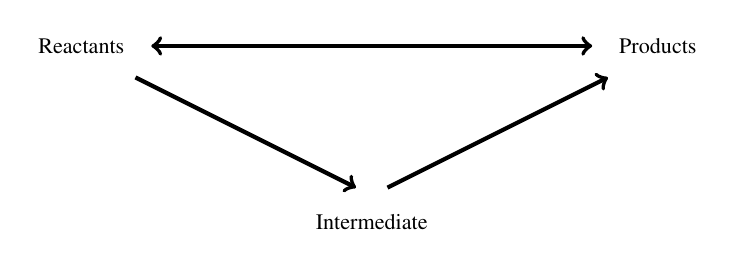
\begin{tikzpicture}
   \node[below] at (4,1) {Intermediate};
   \node[left] at (1,3) {Reactants};
   \node[right] at (7,3) {Products};

   \draw [<->, line width=1.5pt] (1.2,3) -- (6.8,3);
   \draw [->, line width=1.5pt] (1,2.6) -- (3.8,1.2);
   \draw [<-, line width=1.5pt] (7,2.6) -- (4.2,1.2);
\end{tikzpicture}

\begin{wrapfigure}{r}{0.35\textwidth}
\vspace{-5.5\baselineskip}\centering
\includegraphics[width=0.35\textwidth]{Figures/Hess Law.jpg}
% \caption{Illustration of Hess's law}
\end{wrapfigure}

\vspace{1ex}
According to Hess's law,
\vspace{-\baselineskip}
$$\Delta H_1 \ = \ \Delta H_2 + \Delta H_3 \ = \ (-111) + (-282.5) \ = \ -393.5  \tab KJ$$

% where $\Delta H_{reaction}$ is the overall change in enthalpy for the desired reaction,$\sum\Delta H_{products}$ represents the sum of the enthalpies of the products, and $\sum\Delta H_{reactants}$ represents the sum of the enthalpies of the reactants. The enthalpy change is usually given as a positive value when heat is absorbed and as a negative value when heat is released.

\vspace{1ex}
The key idea behind Hess's Law is that the enthalpy change of a reaction can be calculated by combining the enthalpy changes of a series of simpler, known reactions. Even when direct measurements are not feasible or available.
\pagebreak



\pagebreak %/*ANCHOR Kinetics
\vspace*{-2\baselineskip}
\Heading{\cyan{Chemical Kinetics}}

\vspace{-0.5\baselineskip}
\Reference[{Question (2 set)}]{all except 1}

\Topic{2. Define order of a reaction, molecularity of a reaction and half-life period. Show that for first order reactions the half-life period is independent of the initial concentration.}

\Topic{3. Deduce the rate expression for second order reaction where both the concentration terms are same. What is half-life period of the second order reaction?}

\Topic{4. Describe the graphical method for the determination of order of reaction.}

\Topic{5. Derive the integrated Arrhenius equation of activation energy. How is the energy of activation determined from the plot?}



\pagebreak %/*ANCHOR Phase diagram
\vspace*{-2\baselineskip}
\Heading{\cyan{Phase diagram}}

\vspace{-0.5\baselineskip}
\Reference[{Question (2 set)}]{(1 or 2) and 3}
\Topic{1. Discuss main features of the phase diagram of water system.}

\Topic{2. Discuss the salient features of phase diagram of carbon dioxide system.}

\Topic{3. Find out the number of degrees of freedom in the following systems:}
\begin{itemize}
   \item Sulphur$(l)$ Sulphur$(vap)$
   \item CaCO\tsub{3}$(s)$ CaO$(s)$ + CO\tsub{2}$(g)$
   \item H\tsub{2}O$(s)$ H\tsub{2}O$(l)$ H\tsub{2}O$(g)$
   \item Na\tsub{2}SO\tsub{4}.10H\tsub{2}O Na\tsub{2}SO\tsub{4} + 10H\tsub{2}O$(g)$
\end{itemize}



\pagebreak %/*ANCHOR pH
\vspace*{-2\baselineskip}
\Heading{\cyan{pH and Buffer}}

\vspace{-0.5\baselineskip}
\Reference[{Question (2 set)}]{(1 or 2) and 3-7}

\vspace{-\baselineskip}
\Topic{1. What are buffer solutions? Derive Henderson's equation to calculate the pH of an acidic buffer and basic buffer solution.}

\textbf{Buffer solution:} A buffer solution is one which maintains its pH fairly constant even upon the addition of small amount of acid or base.

Two common types of buffer solutions are:

\begin{center}
   \begin{tabular}{|p{9cm}|p{9cm}|}\hline
      \thc{Acid buffers}&\thc{Basic buffers}\\\hline
      Consists of a weak acid and its conjugate base, or a mixture of weak acid and its salt.
      & Consists of a weak base and its conjugate acid, or a mixture of weak base and its salt.\\\hline
      e.g: $\mathrm{CH_3COOH + CH_3COONa}$&
      e.g: $\mathrm{NH_4OH + NH_4Cl}$\\\hline
   \end{tabular}
\end{center}


\vspace{1ex}
\Topic{Calculation of the $\mathrm{pH}$ of buffer solutions:}
The $\mathrm{pH}$ of an acid buffer can be calculated from the dissociation constant $ka$, of the weak acid and the concentrations of the acid and salt acid.

The dissociation expression of the weak acid $\mathrm{HA}$, may be represented as

\begin{center}
   $\mathrm{HA} \rightleftharpoons \mathrm{H}^{+}+\mathrm{A}^{-}$
   \vspace{-0.4\baselineskip}
   \begin{align*}
      \text{and, } \ k_a & = \frac{[H+]\left[A^{-}\right]}{[H A]}\\[1ex]
\text{or, } \ \left[H^{+}\right] & = k_a \times \frac{\left[H A^{-}\right]}{\left[A^{-}\right]} \seteqno{1}
   \end{align*}
\end{center}





Thus we can write the equation $(1)$ as,
$$
\left[\mathrm{H}^{+}\right]=k_a \times \frac{[\text{acid}]}{[\text{salt}]} \seteqno{2}
$$
where \ [acid] \ is the initial concentration of the added acid and \ [salt] \ that of the salt used.

Taking negative logs of both sides of the equation $(2)$. We have,
$$
-\log \left[H^{+}\right]=-\log k_a-\log \frac{[\text{acid}]}{[\text{salt}]} \seteqno{3}
$$

but $-\log \left[\mathrm{H}^{+}\right]=\mathrm{pH}$ \tab and \tab $-\log k_a=\mathrm{pk}_a$

Thus from $(3)$, we have
$$
\mathrm{pH} \ = \ \mathrm{pk}_a-\log \frac{[\text{acid}]}{[\text{salt}]} \ = \ \mathrm{pk}_a+\log \frac{[\text{salt}]}{[\text{acid}]}
$$

Hence,
$$
\mathrm{pH} = \ \mathrm{pk}_a+\log \frac{[\text{salt}]}{[\text{acid}]}
$$

This relationship is called the Henderson-Hasselbalch equation or simply Henderson equation.
Similarly, the Henderson-Hesselbalch equation for a basic buffer can be derived and can be stated as,
$$
\mathrm{pOH}=\mathrm{pk}_b+\log \frac{[\text{salt}]}{[\text{base}]}
$$



\Topic{2. Explain with an example why pH of a buffer solution does not change significantly on small addition of acids or bases.}

The key principle behind the buffer action is the ability of the weak acid and its conjugate base to react with added acid or base, minimizing the change in pH.

Let's consider an example of an acetic acid-sodium acetate buffer system. Acetic acid $\mathrm{(CH_3COOH)}$ is a weak acid, and sodium acetate $\mathrm{(CH_3COONa)}$ is its conjugate base.
% The dissociation of acetic acid in water can be represented by the following equilibrium equation:

\begin{figure}[h]
   \centering
   \includegraphics[width=0.35\textwidth]{Figures/Buffer.jpg}
   \caption{Mechanism of Buffer action of an acid buffer}
\end{figure}

\vspace{-\baselineskip}
\Topic{Addition of $(\mathrm{H}^+)$ acid:}
The  $\mathrm{H}^{+}$ ions produced from the dissociation of $\mathrm{HCl}$ are consumed by the acetate ion $\mathrm{(CH_3COO^-)}$ to form acetic acid $\mathrm{(CH_3COOH)}$. As a result, the increase in  $\mathrm{H}^{+}$ concentration is counteracted by the formation of acetic acid, preventing a significant change in pH.

\Topic{Addition of $(\mathrm{OH^-})$ base:}
When $\mathrm{OH^-}$ is added to the buffer solution, the additional $\mathrm{OH^-}$ ions combine with $\mathrm{H}^{+}$ ions of the buffer to form water molecules. As a result the equilibrium shifts to the right to produce more $\mathrm{H}^{+}$ ions till all the $\mathrm{OH^-}$ ions arce neutralised and the original buffer pH restored.


\pagebreak %/*ANCHOR Electrical
\vspace*{-2\baselineskip}
\Heading{\cyan{Electrical properties of Solution}}

\vspace{-0.5\baselineskip}
\Reference[{Question (1 set)}]{all except 2}

\Topic{1. Define conductance, specific conductance, equivalent conductance and molar
conductance.}

\textbf{Conductance:} Conductance is a measure of how easily electric charges can move through a material like metals and non-metals.

\begin{center}
   $G = \frac{1}{R}$ \tab ohm$^{-1}$ 
\end{center}

\textbf{Specific conductance:} Specific conductance is defined as the conductance of a solution between two electrodes placed 1 cm apart, with an area of 1 sq.cm.

\begin{center}
$\scalebox{1.5}{$\kappa$} = \frac{1}{\rho} = \frac{1}{R} \times \frac{l}{A}$ \tab ohm$^{-1}$ cm$^{-1}$ 

where, R= Resistance, l= length and A= cross-sectional area
\end{center}

\vspace{1ex}
\textbf{Equivalent conductance:} Equivalent conductance refers to the conductivity of an solution containing one equivalent of the electrolyte.

\begin{center}
   $\Lambda_{eq} = \frac{\scalebox{1.2}{$\kappa$} \times 1000}{N}$ \tab ohm$^{-1}$ cm$^{2}$ eq$^{-1}$

   \begin{tabular}{ll}
      Where, & \scalebox{1.5}{$\kappa$} is specific conductance of the solution.\\
       & $N$ is normality of solution.
   \end{tabular}
\end{center}

\textbf{Molar conductance:} Molar conductance refers to  the conductivity of a solution containing 1 mole of electrolyte in a specified volume.

\begin{center}
   $\mu = \frac{\scalebox{1.2}{$\kappa$} \times 1000}{M}$ \tab  ohm$^{-1}$ cm$^{2}$ mol$^{-1}$

   \begin{tabular}{ll}
      Where, & \scalebox{1.5}{$\kappa$} is specific conductance of the solution.\\
       & $M$ is molarity of solution.
   \end{tabular}
\end{center}

\pagebreak
\vspace*{-\baselineskip}
\Topic{3. "On progressive dilution, specific conductance of an electrolyte decreases but molar conductance increases" discuss.}

When an electrolyte is diluted, the number of ions per unit volume decreases, leading to a decrease in specific conductance. This is because the conductivity of a solution depends on the number of ions available to carry an electric current. As the concentration of the electrolyte decreases, the number of ions available to conduct electricity decreases, resulting in a lower specific conductance.

\vspace{1ex}
On the other hand, molar conductance is a measure of the conductivity of the electrolyte per unit concentration. As the solution is progressively diluted, the average distance between ions increases. This reduces the electrostatic interactions and ion-ion interference, allowing the ions to move more freely in the solution, resulting in an increase in molar conductance.


\vspace{1ex}
In summary, as an electrolyte solution is progressively diluted, the decrease in ion concentration leads to a decrease in specific conductance. However, the weakening of ion-ion interactions allows for greater ion mobility and an increase in molar conductance.
\end{document}

\vspace{1ex}
% Molar conductance, on the other hand, is a measure of the conductivity of an electrolyte solution based on the number of moles of the electrolyte present. It takes into account the individual ion conductivities and their respective concentrations. When an electrolyte is diluted, the ion-ion interactions are weakened due to increased solvent (typically water) molecules coming between the ions. This reduction in ion-ion interactions results in increased ion mobility and, consequently, an increase in molar conductance.
